\documentclass[12pt, a4paper]{report}
\usepackage{graphicx}
\usepackage[english]{babel}
\usepackage{amsthm}
\usepackage{amssymb}
\usepackage{amsmath}
\usepackage{algorithm}
\usepackage{algpseudocode}

\newtheorem{theorem}{Theorem}[section]
\newtheorem{corollary}{Corollary}[theorem]
\newtheorem{lemma}[theorem]{Lemma}
\theoremstyle{remark}
\newtheorem*{remark}{Definition}

\title{Software Engineering II}
\author{Christian Rossi}
\date{Academic Year 2023-2024}

\begin{document}

\maketitle

\newpage

\begin{abstract}
    The objective of the course is to teach the principals methods and processes of software engineering needed to develop complex and qualitative software.
    \par
    The course covers the following arguments:
    \begin{itemize}
        \item Software process and its organization.
        \item Modelling languages.
        \item Requirements analysis and definition.
        \item Software development methods and tools.
        \item Approaches for verify and validate the software.
    \end{itemize}
\end{abstract}

\newpage

\tableofcontents

\newpage

\chapter{Introduction}
\section{Definition}
    Software engineering is important because software is everywhere and our society is now totally dependent on software-intensive systems. Software engineering deals with software: 
    \begin{itemize}
        \item Large and complex.
        \item Built by teams.
        \item That exists in many versions.
        \item That lasts many years.
        \item That undergo changes.
    \end{itemize}
    All of this can be resumed as multi-person construction of multi-version software. 
    \begin{remark}
        \emph{Software engineering} is a methodological and managerial discipline concerning the systematic production and maintenance of software products that are developed and maintained within anticipated and controlled time and cost limits.
    \end{remark}
    \par
    The programmer develops a complete software and works on known specifications individually. Instead, the software engineer identifies requirements and develop specifications, designs components that will be combined with others and works in a team. The main skills of a software engineer are: technical, managerial, cognitive, organizational.
\section{History}
    Initially, the software was considered as an art. The computers were used for computing to solve mathematical problems and the designers were also the users. The first programs were created with low-level languages and had high resources constraints. 
    \par
    When the request for new custom software exploded the art became a craft: the developer started to create programs also for the people with new high-level languages. At the end of this period there were a "software crisis" due to increasing software complexity and lack of effective software development techniques. 
    \par
    To solve this problem in 1968 was defined the term \emph{software engineering} in a NATO conference. The main focuses of this conference was on: 
    \begin{itemize}
        \item Development of software and standards.
        \item Planning and management.
        \item Automation.
        \item Modularization.
        \item Quality verification.
    \end{itemize}
\section{The process and product}
    The developing of a software program needs a process. Both software and processes have a quality and the software engineer needs to reach the optimal quality because the process modifies the final output.
    \par
    The software is different from traditional types of products because it is: 
    \begin{enumerate}
        \item Intangible (difficult to describe and evaluate).
        \item Malleable.
        \item Human intensive (does not involve any trivial manufacturing process).
    \end{enumerate}
    The quality of the software is influenced by the following variables: development technology, process quality, people quality, cost, time and schedule. The software quality attribute are:
    \begin{itemize}
        \item Correctness: software is correct if it satisfies the specifications.
        \item Reliability: probability of absence of failures for a certain time period.
        \item Robustness: software behaves reasonably even in unforeseen circumstances.
        \item Performance: efficient use of resources.
        \item Usability: expected users find the system easy to use.
        \item Maintainability.
        \item Reusability: similar to maintainability but applies to components.
        \item Portability: adaption to different target environments.
        Interoperability: coexist and cooperate with other applications. 
    \end{itemize}
    The process quality attribute are:
    \begin{itemize}
        \item Productivity.
        \item Unity of effort (person month).
        \item Delivered item (lines of code and function points).
        \item Timeliness: ability to respond to change requests in a timely fashion.
    \end{itemize}
\section{Development process}
    Initially there were no reference model, so it was simple code$\&$fix. As a reaction to the software crisis mentioned before it became necessary to have a model. The first complete model was the "waterfall". The key requirements of this model are:
    \begin{enumerate}
        \item Identify phases and activities.
        \item Force linear progression from a phase to the next (without returns).
        \item Standardize outputs from each phase.
        \item Software is considered like manufacturing.
    \end{enumerate}
    After this model many other flexible processes were proposed: iterative models, agile movement and DevOps.
    \begin{figure}
        \centering
        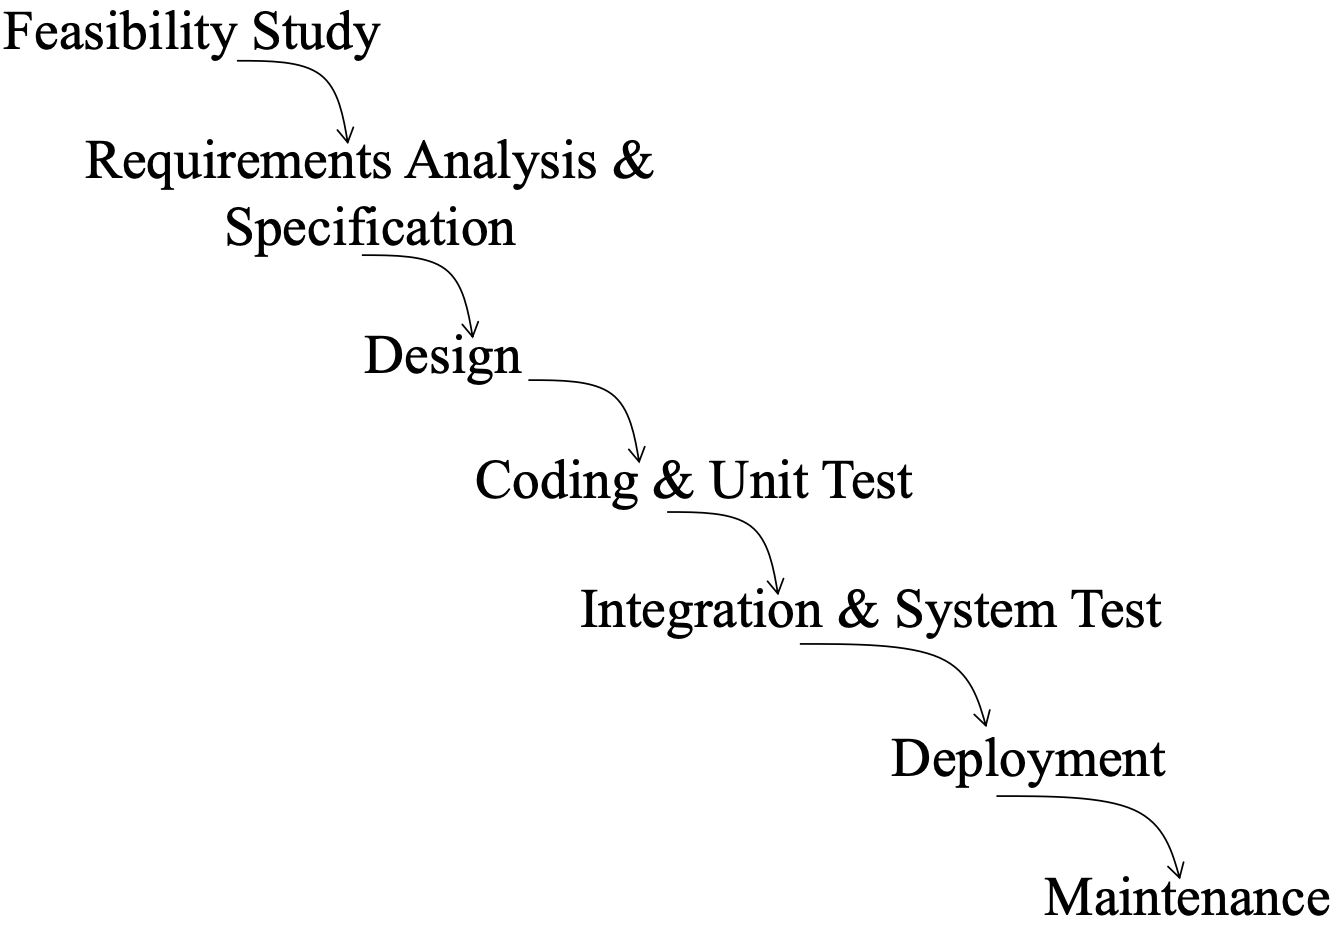
\includegraphics[width=0.5\linewidth]{images/waterfall.png}
        \caption{Waterfall process model}
    \end{figure}
    The main phases shown in the image are:
    \begin{enumerate}
        \item Feasibility study and project estimation: determines wheather the project should be started, the possible alternatives and needed resources. This phase produces a \emph{Feasibility Study Document} which contains: preliminary problem description, scenarios describing possible solutions, cost and schedule for the different alternatives.
        \item Requirement analysis and specification: analyze the domain in which the application takes place, identify requirements and derive specification for the software. This phase produces \emph{Requirement Analysis and Specification Document}.
        \item Design: defines the software architecture (components, relation and interactions among components). The goal is to support concurrent development and separate responsibilities. It produces the \emph{Design Document}.
        \item Coding and unit test: each module is implemented and tested. Inspection can be used as an additional quality assurance approach. Programs include their documentation. 
        \item Integration and system test: the modules are integrated into systems and integrated systems are tested. This phase and the previous may be integrated in an incremental implementation scheme. 
        \item Deployment.
        \item Maintenance: the maintenance can be:
        \begin{itemize}
            \item Corrective: deals with the repair of faults or defects found.
            \item Adaptive: consist of adapting software to changes in the environment.
            \item Perfective: deals with accommodating to new or changed user requirements.
            \item Preventive: concerns activities aimed at increasing the system's maintainability. 
        \end{itemize}
    \end{enumerate}
    \begin{figure}
        \centering
        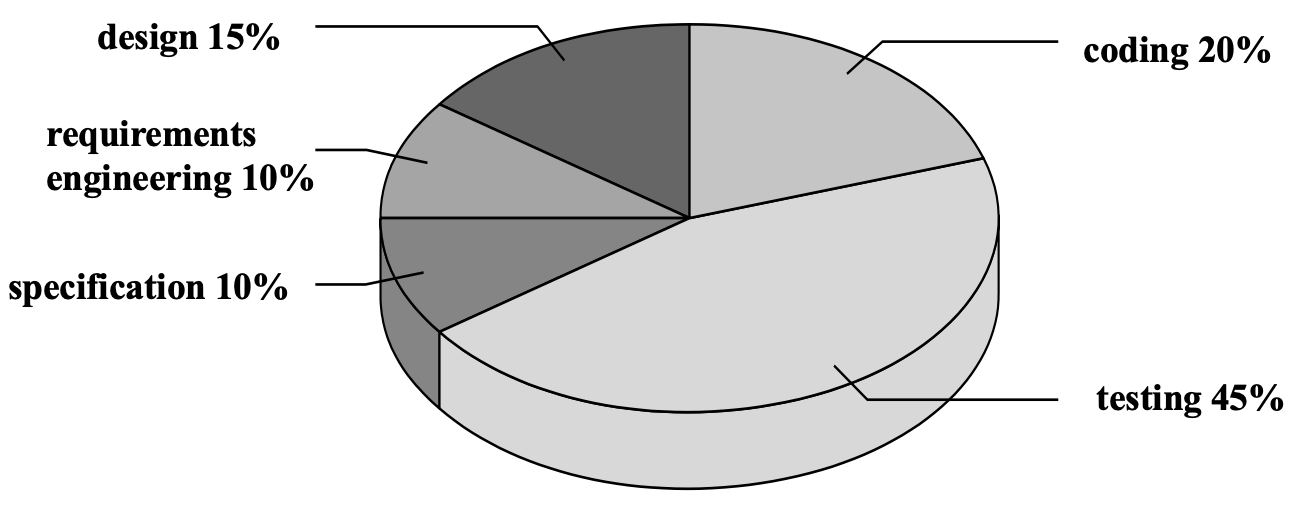
\includegraphics[width=1\linewidth]{images/effort.png}
        \caption{Effort in each phase}
    \end{figure}
    \par
    The principal problems with software evolution are:
    \begin{itemize}
        \item It is almost never anticipated and planned.
        \item Software is very easy to change (changes applied directly to the code that causes inconsistent state of project documents).
    \end{itemize}
    To face properly the evolution we need a good engineering practice that consist in two main steps: modify the design and then change the implementation and apply changes consistently in all documents. In fact, one of the main goal of software engineering is to create software that must be designed to accommodate future changes reliably and cheaply. 
    \par
    Waterfall model is a black-box system because the company that requests the software makes requirements and doesn't interact during the development phase. If we need more transparency with the customer we need to use a different development model (that allows the customer to give feedback regularly). With every interaction with the customer is possible to check two main things:
    \begin{itemize}
        \item Validation: check if the product follows the customer's requests.
        \item Verification: check if the product works in the right way.
    \end{itemize}
    \par
    The idea of flexible process is to adapt to changes, in particular the requirements and specification. The idea is to have incremental processes and be able to get feedback on increments. They exists in many forms, for example: SCRUM, extreme programming, incremental releases and rapid prototyping, DevOps, $\dots$
    
\newpage

\chapter{Requirements engineering}
\section{Definition}
    The primary measure of success of a software system is the degree to which it meets the purpose for which it was intended.
    \begin{remark}
        Software systems \emph{requirements engineering} is the process of discovering that purpose, by identifying stakeholders and their needs, and documenting these in a form that is amenable to analysis, communication, and subsequent implementation. 
    \end{remark}
    The important issues of this phase are: identify stakeholders, identify their needs, produce documentation and analyse, communicate and implement requirements. Another possible definition is the following. 
    \begin{remark}
        \emph{Requirements engineering} is the branch of software engineering concerned with the 
        \begin{itemize}
            \item real-world goals for,
            \item function of, and
            \item constraints on
        \end{itemize}
        software systems. It is also concerned with the relationship of these factors to precise specifications of software engineering behaviour, and to their evolution over time and across software families. 
    \end{remark}
\section{Importance and difficulties}
    The requirements given from the customer can be classified in three main types:
    \begin{itemize}
        \item Functional: describes the interaction between the system and its environment independent from implementation. They are the main goals that the software has to fulfill.
        \item Nonfunctional: user visible aspects of the system not directly related to functional behaviour.
        \item Constraints: imposed by the client or the environment in which the system operates.
    \end{itemize}
    The nonfunctional requirements are constraints on how functionality has to be provided to the end user. They are independent of application domain but the application domain determines: their relevance and their prioritization. They are also called Quality of Service attribute. 
    \begin{figure}
        \centering
        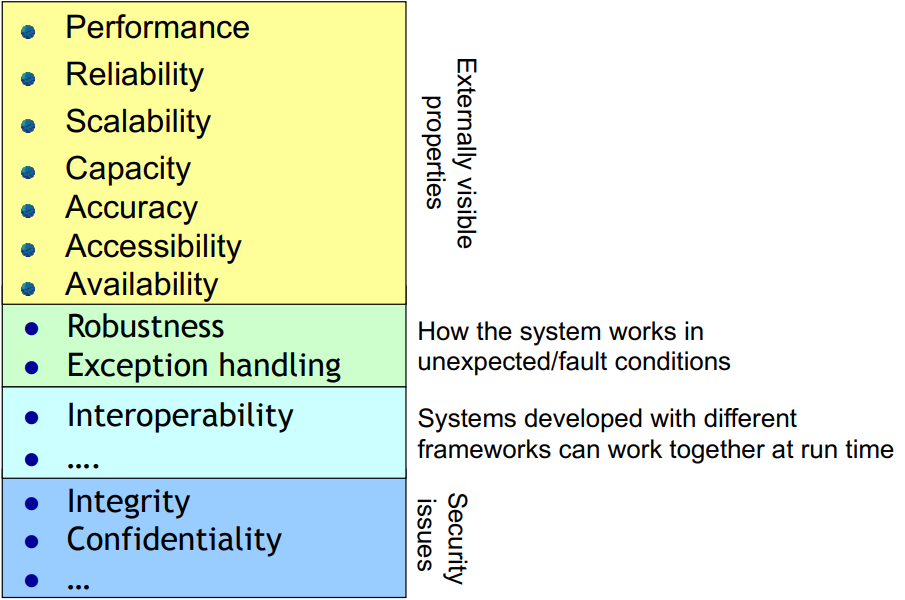
\includegraphics[width=1\linewidth]{images/QoS.png}
        \caption{Some relevant QoS characteristics}
    \end{figure}
\section{The requirement engineering process}
    Poor requirements are ubiquitous. Requirement engineering is also hard and critical because a problem with the initial phases can be up to two hundred times costly in the final phase. 
    \begin{figure}
        \centering
        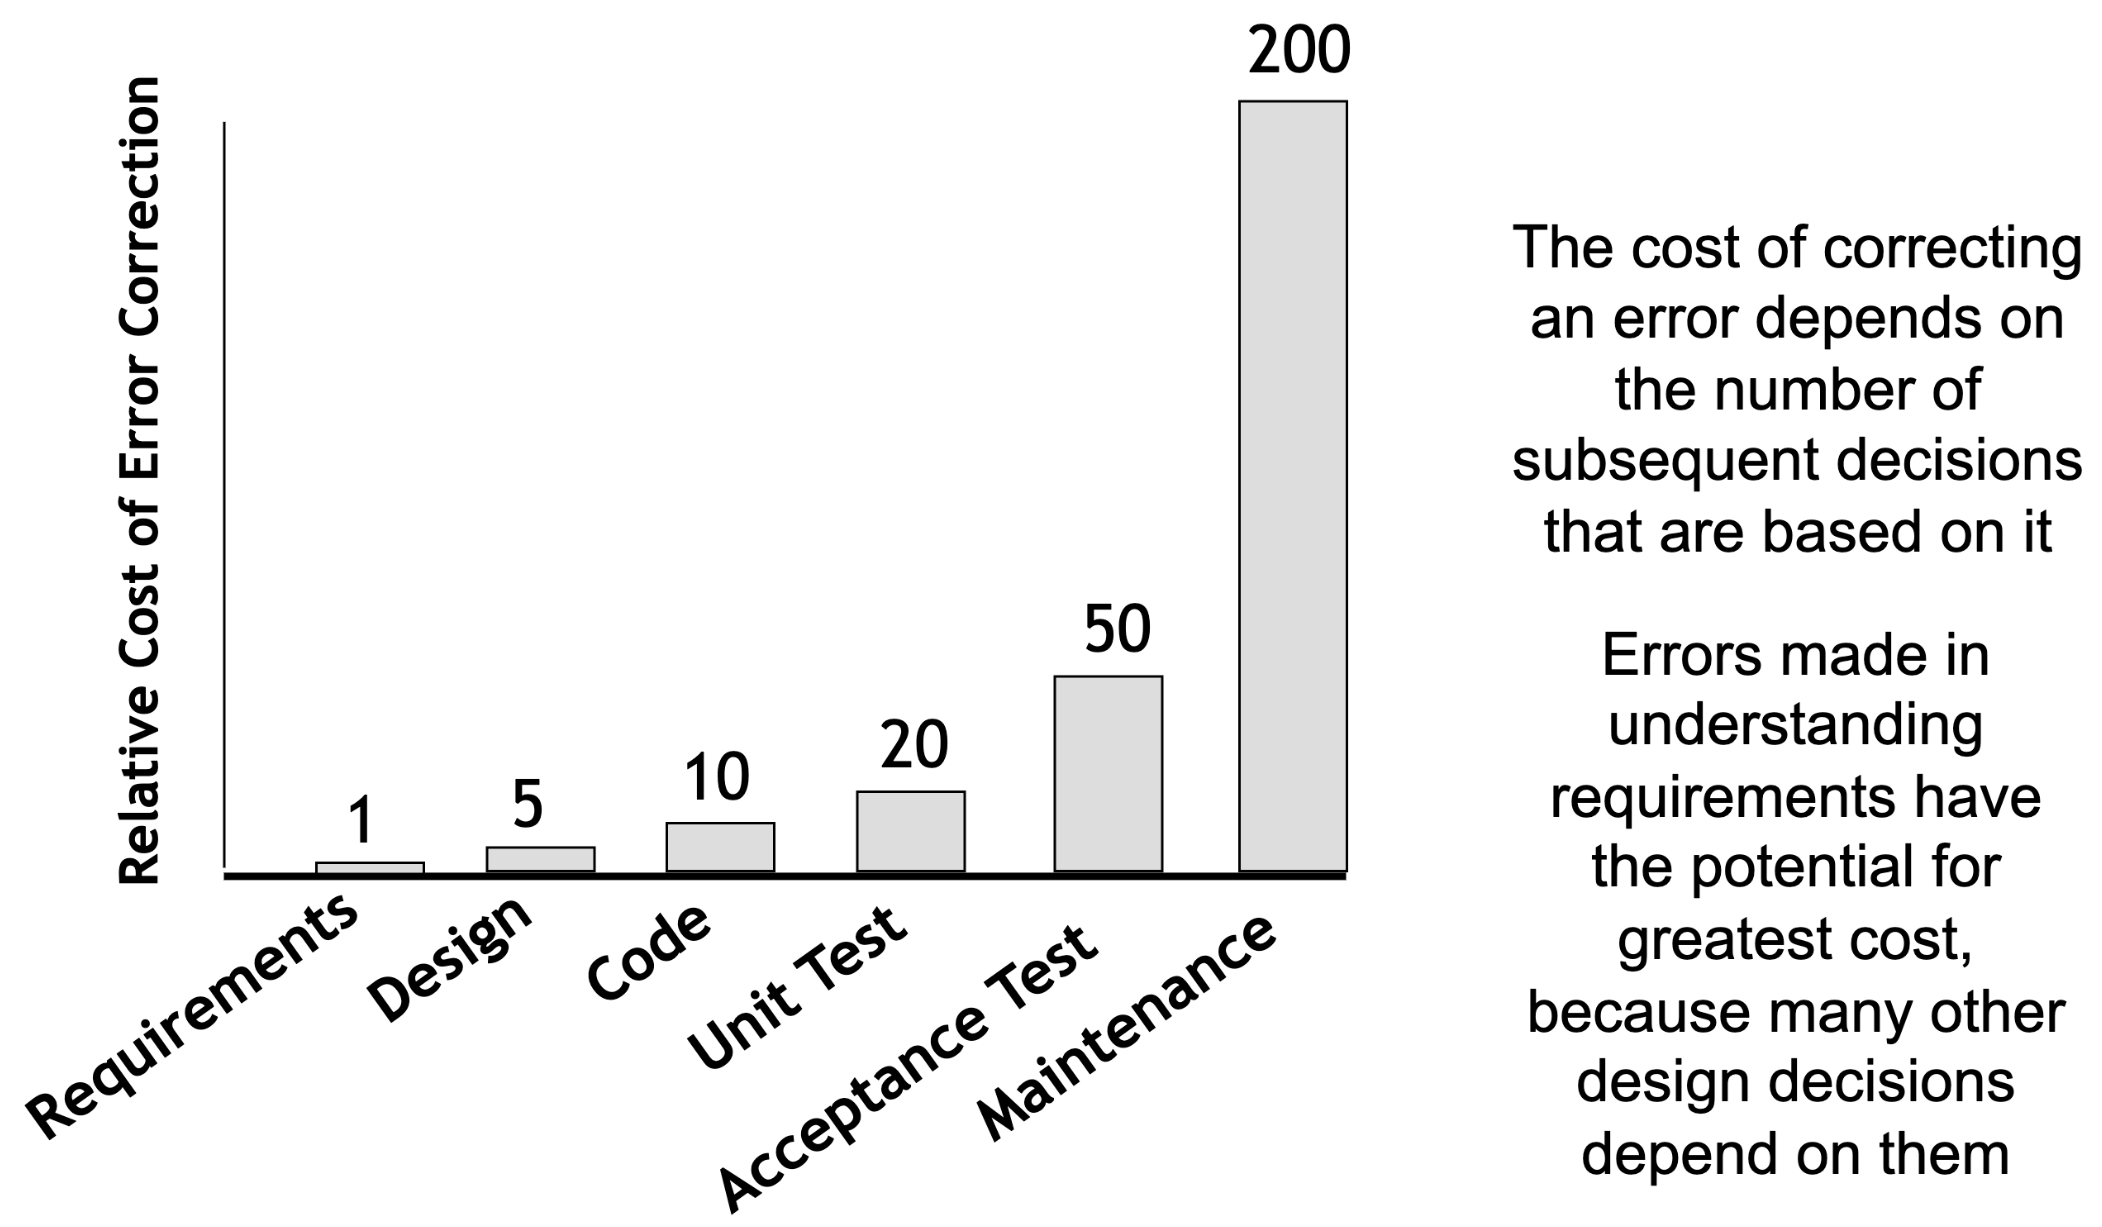
\includegraphics[width=1\linewidth]{images/requirements.png}
        \caption{Cost of late correction [Boehm, 1981]}
    \end{figure}
    Requirement engineering is so complex because of: composite systems. more than one system, multiple abstraction levels, multiple concerns and multiple stakeholders with different background.
    \par
    The requirement engineers needs to: 
    \begin{itemize}
        \item Eliciting information (project objectives, context and scope; domain scope and requirements).
        \item Modelling and analysis (goals, objects, use cases and scenarios).
        \item Communicating requirements (analysis feedback, RASD document, system prototypes).
        \item Negotiating and agreeing requirements (handling conflicts and risks; helping in requirement selection and prioritization).
        \item Managing and evolving requirements (managing requirements during development: backward and forward traceability; managing requirements changes and their impacts).
    \end{itemize}
\section{Understanding world-machine relationship}
    The machine indicates the portion of system to be developed, while world indicates the portion of the real-world affected by the machine. The purpose of the machine is always in the world. 
    \par
    Requirements engineering is concerned with phenomena occurring in the world as opposed to phenomena occurring inside the machine. We can say that requirements models are models of the world. 
    \par
    Some world phenomena are shared with the machine. This type of phenomena can be: 
    \begin{itemize}
        \item Controlled by the world and observed by the machine.
        \item Controlled by the machine and observed by the world.
    \end{itemize}
    \begin{figure}
        \centering
        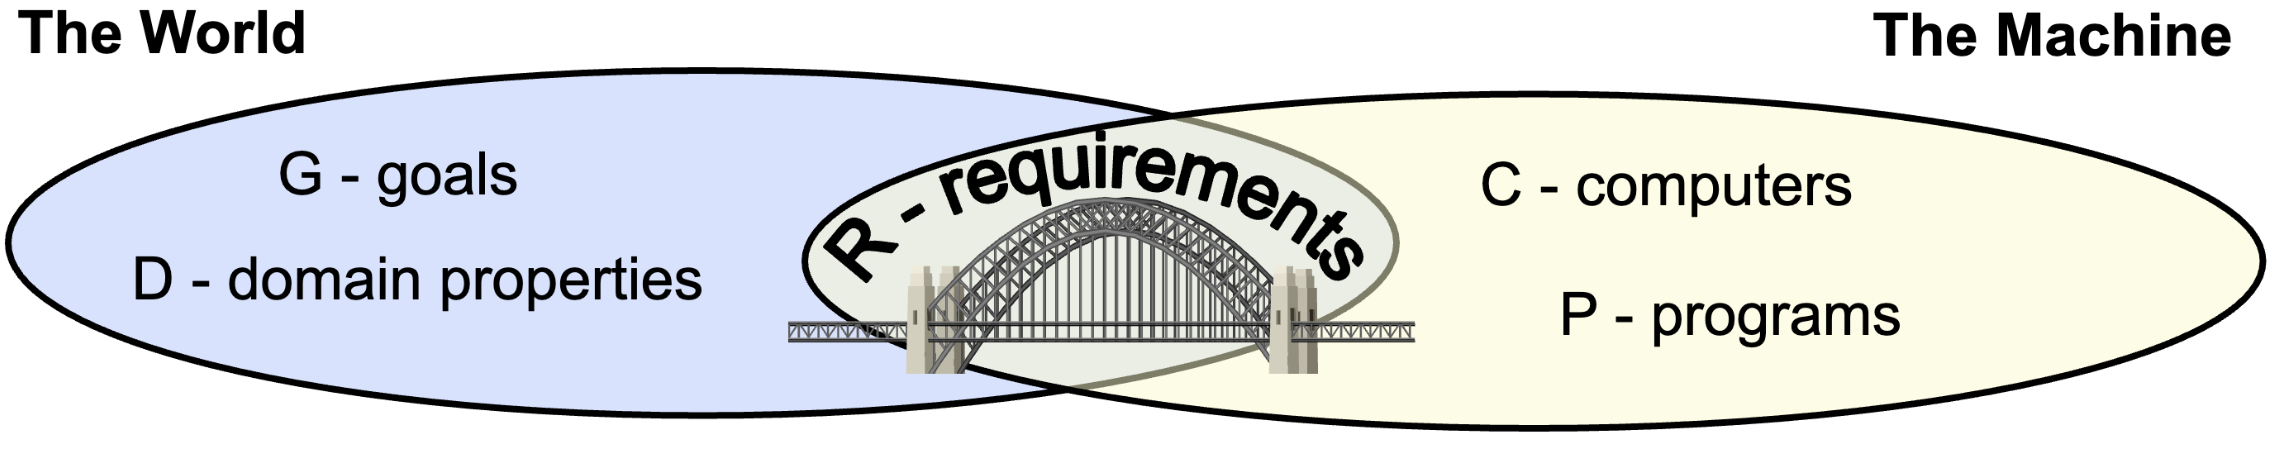
\includegraphics[width=1\linewidth]{images/worldmachine.png}
        \caption{Goals, domain assumptions, and requirements}
    \end{figure}
    Goals are prescriptive assertions formulated in terms of world phenomena (not necessarily shared). Domains properties/assumptions are descriptive assertions assumed to hold in the world. Requirements are prescriptive assertions formulated in terms of shared phenomena. 
    \par 
    The requirements $R$ are complete if: 
    \begin{itemize}
        \item $R$ ensures satisfaction of the goals $G$ in the context of the domain properties $D$, this means that $R\land D \models G$.
        \item $G$ adequately capture all the stakeholders' needs.
        \item $D$ represent valid properties/assumptions about the world.
    \end{itemize}
\section{Elicitation of requirements}
    The complexity in requirement engineering can be coped with:
    \begin{itemize}
        \item Adopting different approaches and strategies and combining the results reached with all of them.
        \item Being as close as possible to stakeholders.
        \item Letting stakeholders describing their viewpoints.
    \end{itemize}
    The scenario can be generalized in term of:
    \begin{itemize}
        \item Participation actors.
        \item Describe the entry condition.
        \item Describe the flow of events.
        \item Describe the exit condition.
        \item Describe exceptions.
        \item Describe special requirements.
    \end{itemize}
\section{Modeling requirements}
    \begin{remark}
        A \emph{model} is a representation in a certain medium of something in the same or another medium. The model captures the important aspects of the thing being modeled and simplifies or omits the rest. 
    \end{remark}
    The reality $R$ is composed by: real things, people, processes and relationship. The model $M$ is an abstraction of things, people, processes and relationship between these abstraction. 
    \par
    The reality needs to be interpreted ($I$) with a mapping function. To have a good model the relationships that are valid in the reality $R$ need to be valid also in the model $M$.
    \begin{figure}
        \centering
        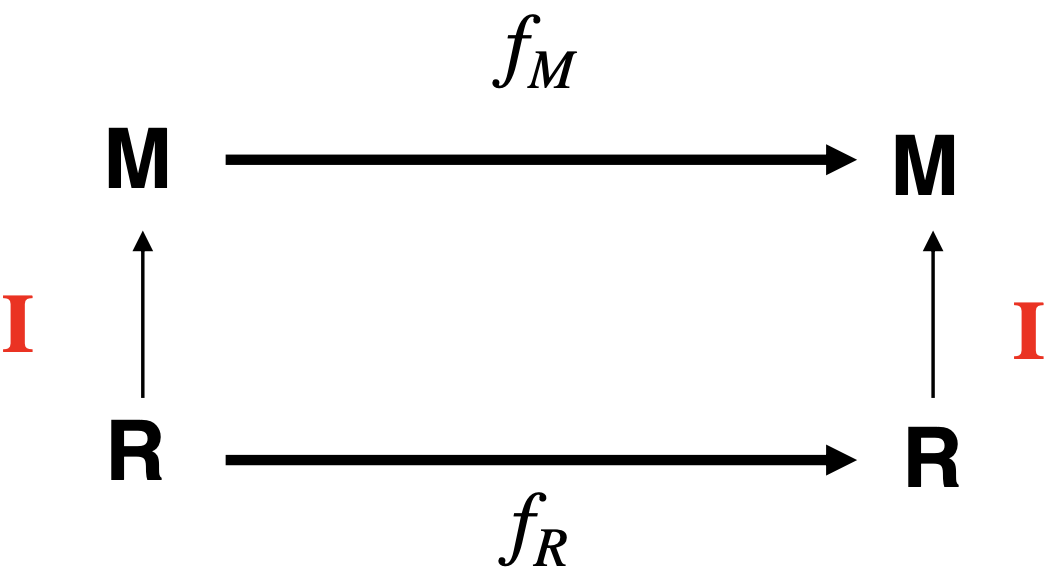
\includegraphics[width=1\linewidth]{images/modeling.png}
        \caption{Relationship between model $M$ and reality $R$}
    \end{figure}
    The software models are used for: 
    \begin{itemize}
        \item Capture and precisely state requirements and domain knowledge.
        \item Think about the design of a software system Generate usable work products.
        \item Give a simplified view of complex systems Evaluate and simulate a complex system.
        \item Generate potential configurations of systems.
    \end{itemize}
    The principal modeling issues are coherence (different views of the system must be coherent) and variation in interpretation and ambiguity (define where different interpretation of the model are acceptable).
    \par
    In requirements engineering we should only model:
    \begin{itemize}
        \item The objects and people that are of interest for the given problem.
        \item The relevant phenomena.
        \item The goals, requirements, and domain assumptions.
    \end{itemize}
    The tool that we can use for modeling are: 
    \begin{itemize}
        \item Natural language (English, Italian, $\dots$):
        \begin{itemize}
            \item Pros: simplicity of use.
            \item Cons: high level of ambiguity, it is easy to forget to include relevant information.
        \end{itemize}
        \item Formal language (FOL, Alloy, Z, $\dots$):
        \begin{itemize}
            \item Pros: possibility to use tool to support analysis and validation, the approach forces the user in specifying all relevant details.
            \item Cons: you need to be expert in the use of the language.
        \end{itemize}
        \item Semi-formal language (UML):
        \begin{itemize}
            \item Pros: simpler than a formal language, impose some kind of structure in the models.
            \item Cons: not amenable for automated analysis, some level of ambiguity.
        \end{itemize}
        \item Mixed approach: use a semi-formal language for the basics. Comment and complement the semi-formal models with explanatory informal text. use a formal language for the most critical parts.
    \end{itemize}
\section{Use cases and requirements}
    The main steps when formulating use cases are: 
    \begin{enumerate}
        \item Name the use case
        \item Find the actors: generalize the concrete names to participating actors.
        \item Concentrate on the flows of events, entry and exit condition using natural language.
        \item Focus on exceptional cases and special requirements.
    \end{enumerate}
    Each use case may lead to one or more requirements.
    \par
    A use case is a flow of events in the system, including interaction with actors. The use cases are initialized by an actor and has a termination condition. 
    \begin{remark}
        The \emph{use case model} is the set of all use cases specifying the complete functionality of the system. 
    \end{remark}
    \begin{remark}
        A \emph{use case association} is a relationship between use cases. The principal types of use case association are: 
        \begin{itemize}
            \item Include(a use case uses another use case).
            \item Extends (a use case extends another use case).
            \item Generalization (an abstract use case has several different specializations).
        \end{itemize}
    \end{remark}
    \begin{figure}
        \centering
        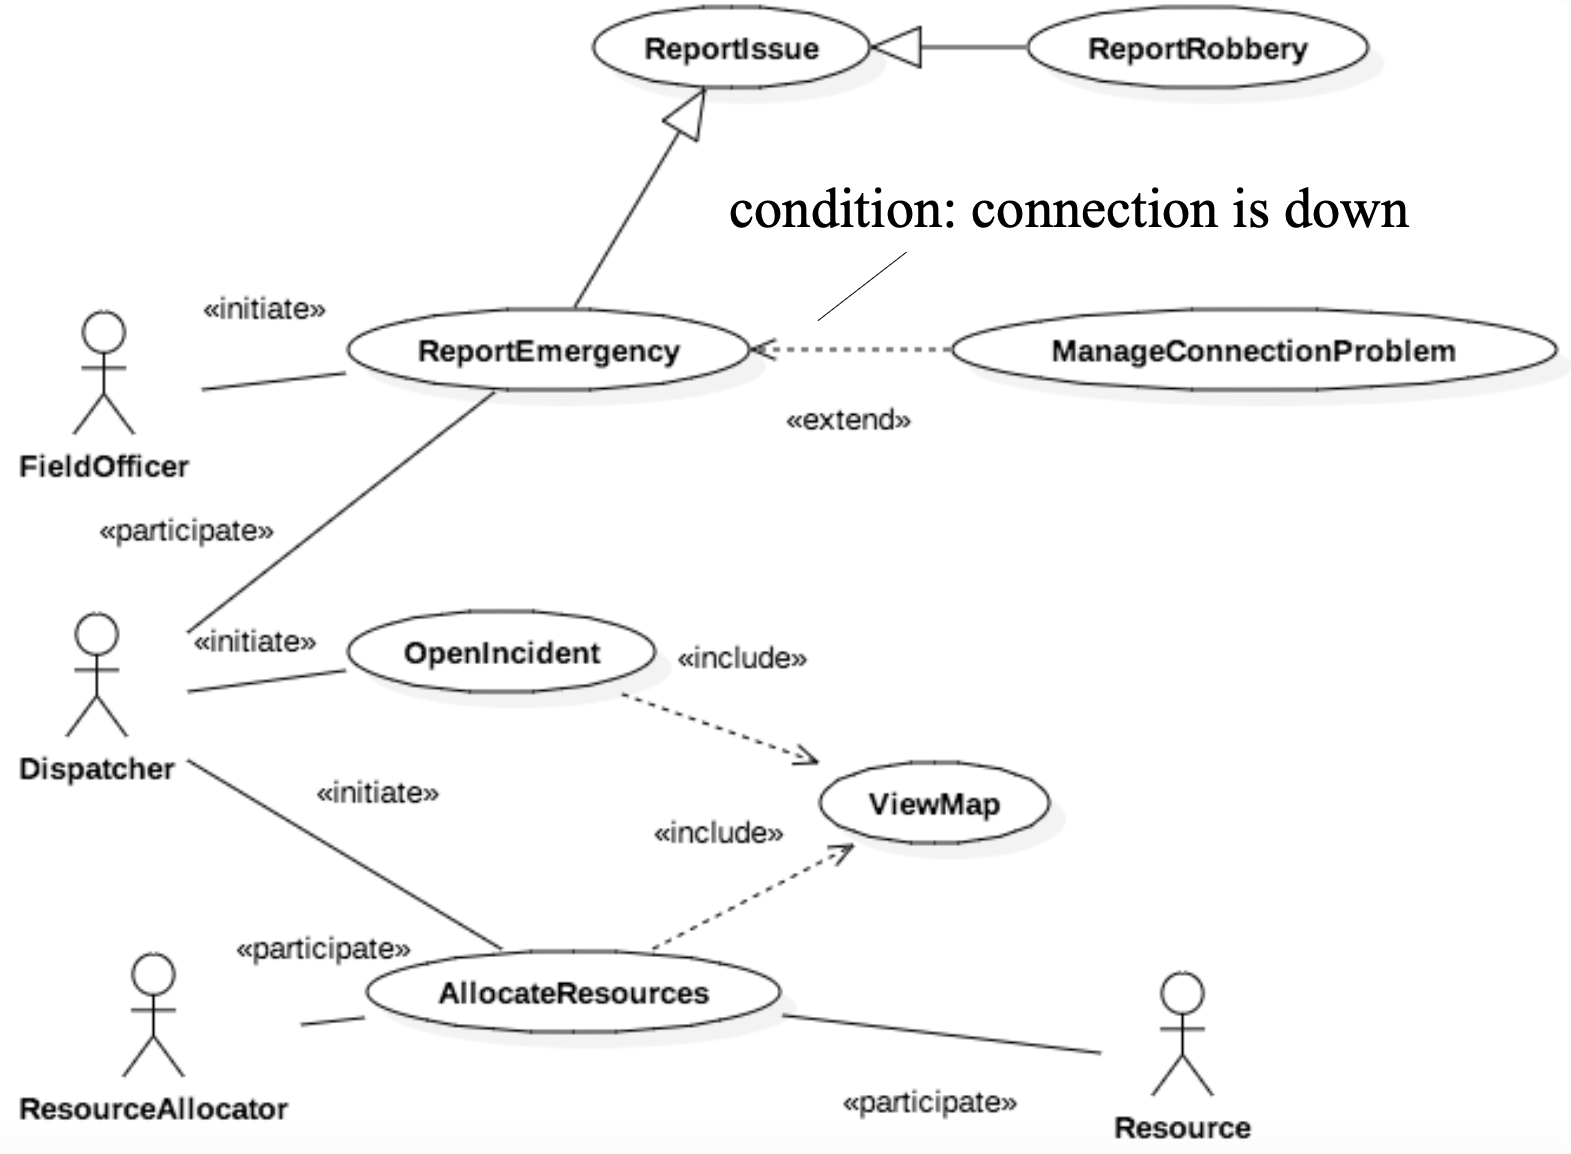
\includegraphics[width=0.5\linewidth]{images/usecase.png}
        \caption{Use case model example}
    \end{figure}
\section{Requirements-level class diagrams}
    The requirements-level class diagrams are conceptual models for the application domain. They may model objects that will not be represented in the software-to-be. Usually, the do not attach operations to objects: it's best to postpone this kind of decisions until software design. 
    \par
    To find objects and classes we need to:
    \begin{itemize}
        \item Analyze any description of the problem and application domain you may have.
        \item Analyze your scenarios and use cases descriptions.
    \end{itemize}
    Finding objects is the central piece in object modeling. A possible tool to use in the analysis is the Abbott Textual Analysis also called noun-verb analysis: nouns are good candidates for classes and verbs are good candidates for associations and operations. 
    \begin{figure}
        \centering
        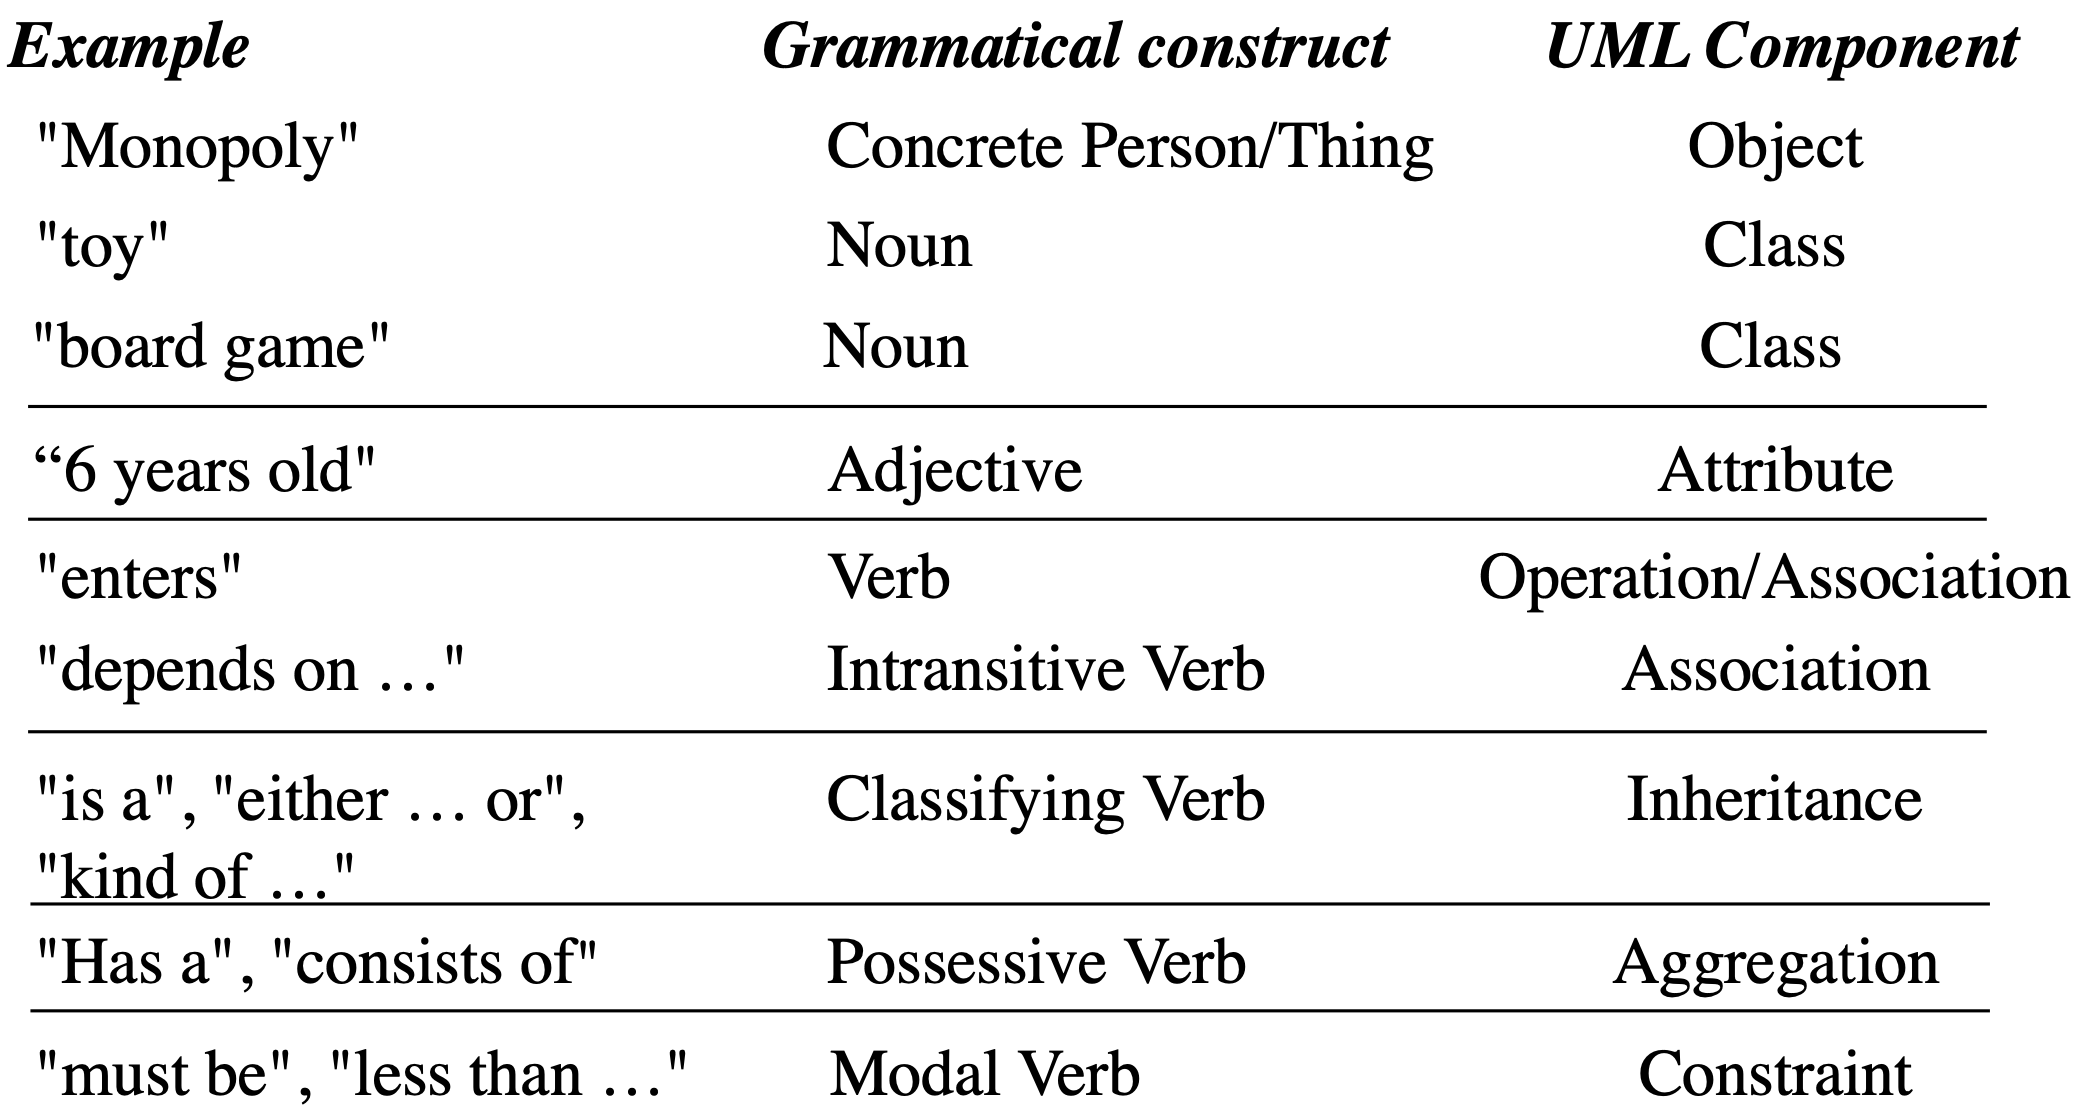
\includegraphics[width=0.5\linewidth]{images/Abbott.png}
        \caption{Abbott Textual Analysis example}
    \end{figure}
\section{Dynamic modeling}
    The purpose of the dynamic modeling is to supply methods to model interactions, behaviours of participants and workflow. This can be done with: sequence diagram, state machine diagram and activity diagram. Some objects can be found whilst completing those diagrams.
    \par
    The sequence diagram is created following the flow of events in the use case diagram. A sequence diagram is a graphical description of objects participating in a use case scenario using a Directed Acyclic Graph notation.
    The principal rules to create a sequence diagrams are: 
    \begin{itemize}
        \item An event always has a sender and a receiver.
        \item The representation of the event is sometimes called a message.
        \item Find sender and receiver for each event.
    \end{itemize}
    \begin{figure}
        \centering
        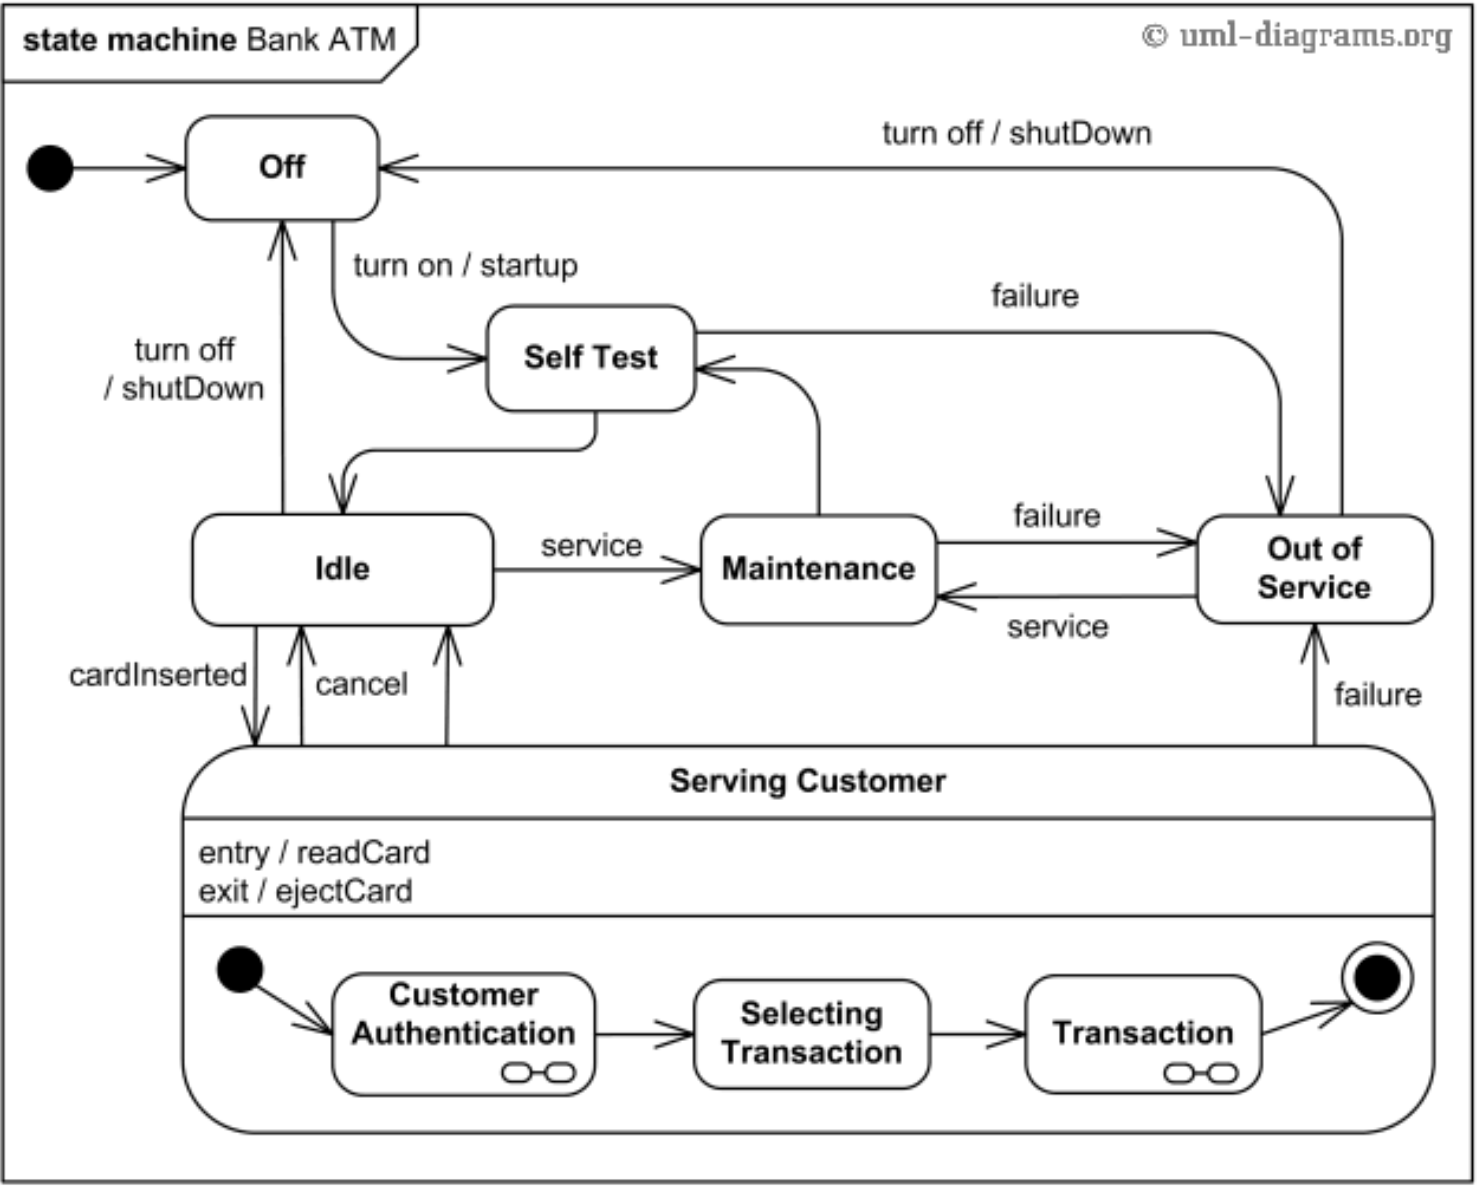
\includegraphics[width=0.5\linewidth]{images/state.png}
        \caption{Example of a state diagram}
    \end{figure}
    \par
    For a good dynamic modeling we ha to construct a model only for classes with significant dynamic behaviour and consider only relevant attributes. We have also to look ate the granularity of the application when deciding on actions and activities and reduce notational clutter.

\newpage

\chapter{Alloy}
\section{Definition}
    Alloy is a formal notation for specifying models of systems and software. It looks like a declarative object oriented language, but also has a mathematical foundation.
    \par
    Alloy comes with a supporting tool to simulate specifications and performs property verification.
    \par
    Alloy has been created to offer an expressive power similar to the Z language as well as the strong automated analysis of the SMW model checker. 
    \par
    Alloy can be used in requirement engineering  to formally describe the domain and its properties, or operations that the machine has to provide. In software design Alloy can be used to formally model components and their interactions. 
\section{Introduction}
    Alloy is a mixture of first order logic and relational calculus. The main elements of this formal language are: 
    \begin{itemize}
        \item Carefully chosen subset of relational algebra (uniform model for individuals, sets and relations; no high-order relations).
        \item Almost no arithmetic.
        \item Modules and hierarchies.
        \item Suitable for small, explanatory specification.
        \item Powerful and fast analysis tool.
    \end{itemize}
\section{Syntax}
    Alloy shows bounded snapshots of the world that satisfy the specification. Allow does bounded exhaustive search for counterexample to a claimed property using SAT.
    \begin{remark}
        \emph{Atoms} are Alloy's primitive entities (indivisible, immutable and uninterpreted). 
    \end{remark}
    \begin{remark}
        \emph{Relations} associate atoms with one another (set of tuples; tuples are sequence of atoms).
    \end{remark}
    The relations in Alloy are typed. The relation type is determined by the declaration of the relation. The basic Alloy relations type are: $none$ (empty set), $univ$ (universal set) and $iden$ (identity relation). The logic operators in Alloy are: 
    \begin{itemize}
        \item Union $\cup$.
        \item Intersection $\&$.
        \item Difference $-$.
        \item Subset $in$.
        \item Equality $=$.
        \item Cross product $\rightarrow$ (similar to a natural join). 
        \item Dot join $.$ or $[\:]$ (the last element of the first relation joins on the corresponding first elements of the second relation, and then removes the element from the relation).
    \end{itemize}
    The possible binary closures on the relations are: 
    \begin{itemize}
        \item Transpose $\sim$ (inverts the order of the elements in the relation).
        \item Transitive $\land$ ($^{\land}r=r+r.r+r.r.r+\dots$). 
        \item Reflexive transitive $*$ ($^{*}r=iden+^{\land}r$)
    \end{itemize}
    The possible restrictions are: 
    \begin{itemize}
        \item Domain restriction $<:$, that restricts the elements on the left side to the set on the right side.
        \item Range restriction $:>$, that is same as before but the relations are inverted. 
        \item Override $++$, that removes the tuples on the left that are in the right relations and adds all the remaining relations of the right relation. 
    \end{itemize}
    The Alloy Boolean operators are the following: negation ($!$ or $not$), conjunction ($\&$ or $and$), disjunction ($\mid \mid$ or $or$), implication ($\implies$ or $implies$), alternative ($,$ or $else$) and bi-implication ($\iff$ or $iff$). The alloy logic quantifiers are: 
    \begin{itemize}
        \item $all$: holds for every element.
        \item $some$: holds for at least one element.
        \item $no$: holds for no elements.
        \item $lone$: holds for at most one element.
        \item $one$: holds for exactly one element.
    \end{itemize}
    To define a relation with a singleton we can use the following declaration: 
    \[x \: : \: m \: e\]
    Where $x$ is the name of the relation, $m$ is the multiplicity of the element (that can be: $set$, $one$, $lone$ or $some$) and $e$ is the name of the element in the relation. If the relation is composed by couple the declaration became like this: 
    \[r \: : \: A \: m \: \rightarrow \: n \: B\]
    Where $r$ is the name of the relation, $A$ and $B$ are the name of the elements with multiplicity $m$ and $n$ respectively.
    \par
    $let$ is used to define a formula or expression that can be reused. Other useful operators are: $\# r$ (that define the number of tuples in $r$), $0,1,\dots$ (integer used to define the value of some variables or constants), $+$ (plus), $-$ (minus), all the comparison operators ($<$, $<=$, $=$, $=>$, $>$). There is also the operator $sum$ that adds all the elements in the selected tuple. 
    
\newpage

\chapter{Requirement analysis and specification}
\section{Structure of a RASD document}
    The RASD has the following purposes: 
    \begin{itemize}
        \item Communicates an understanding of the requirements (application domain and the system to be developed).
        \item Contractual (may be legally binding).
        \item Baseline for project planning and estimation (size, cost and schedule).
        \item Baseline for software evaluation (support system testing, verification and validation activities; should contain enough information to verify weather the delivered system meets requirements).
        \item Baseline for change control (requirements change, software evolves).
    \end{itemize}
    The RASD is used by:
    \begin{itemize}
        \item Customers and users (interested in high level description of functionalities).
        \item System analyst and requirement analyst (specification of other system to inter-relate).
        \item Developers and programmers (implementation).
        \item testers (check if requirements are met).
        \item Project managers (control the development process).
    \end{itemize}
    \begin{figure}
        \centering
        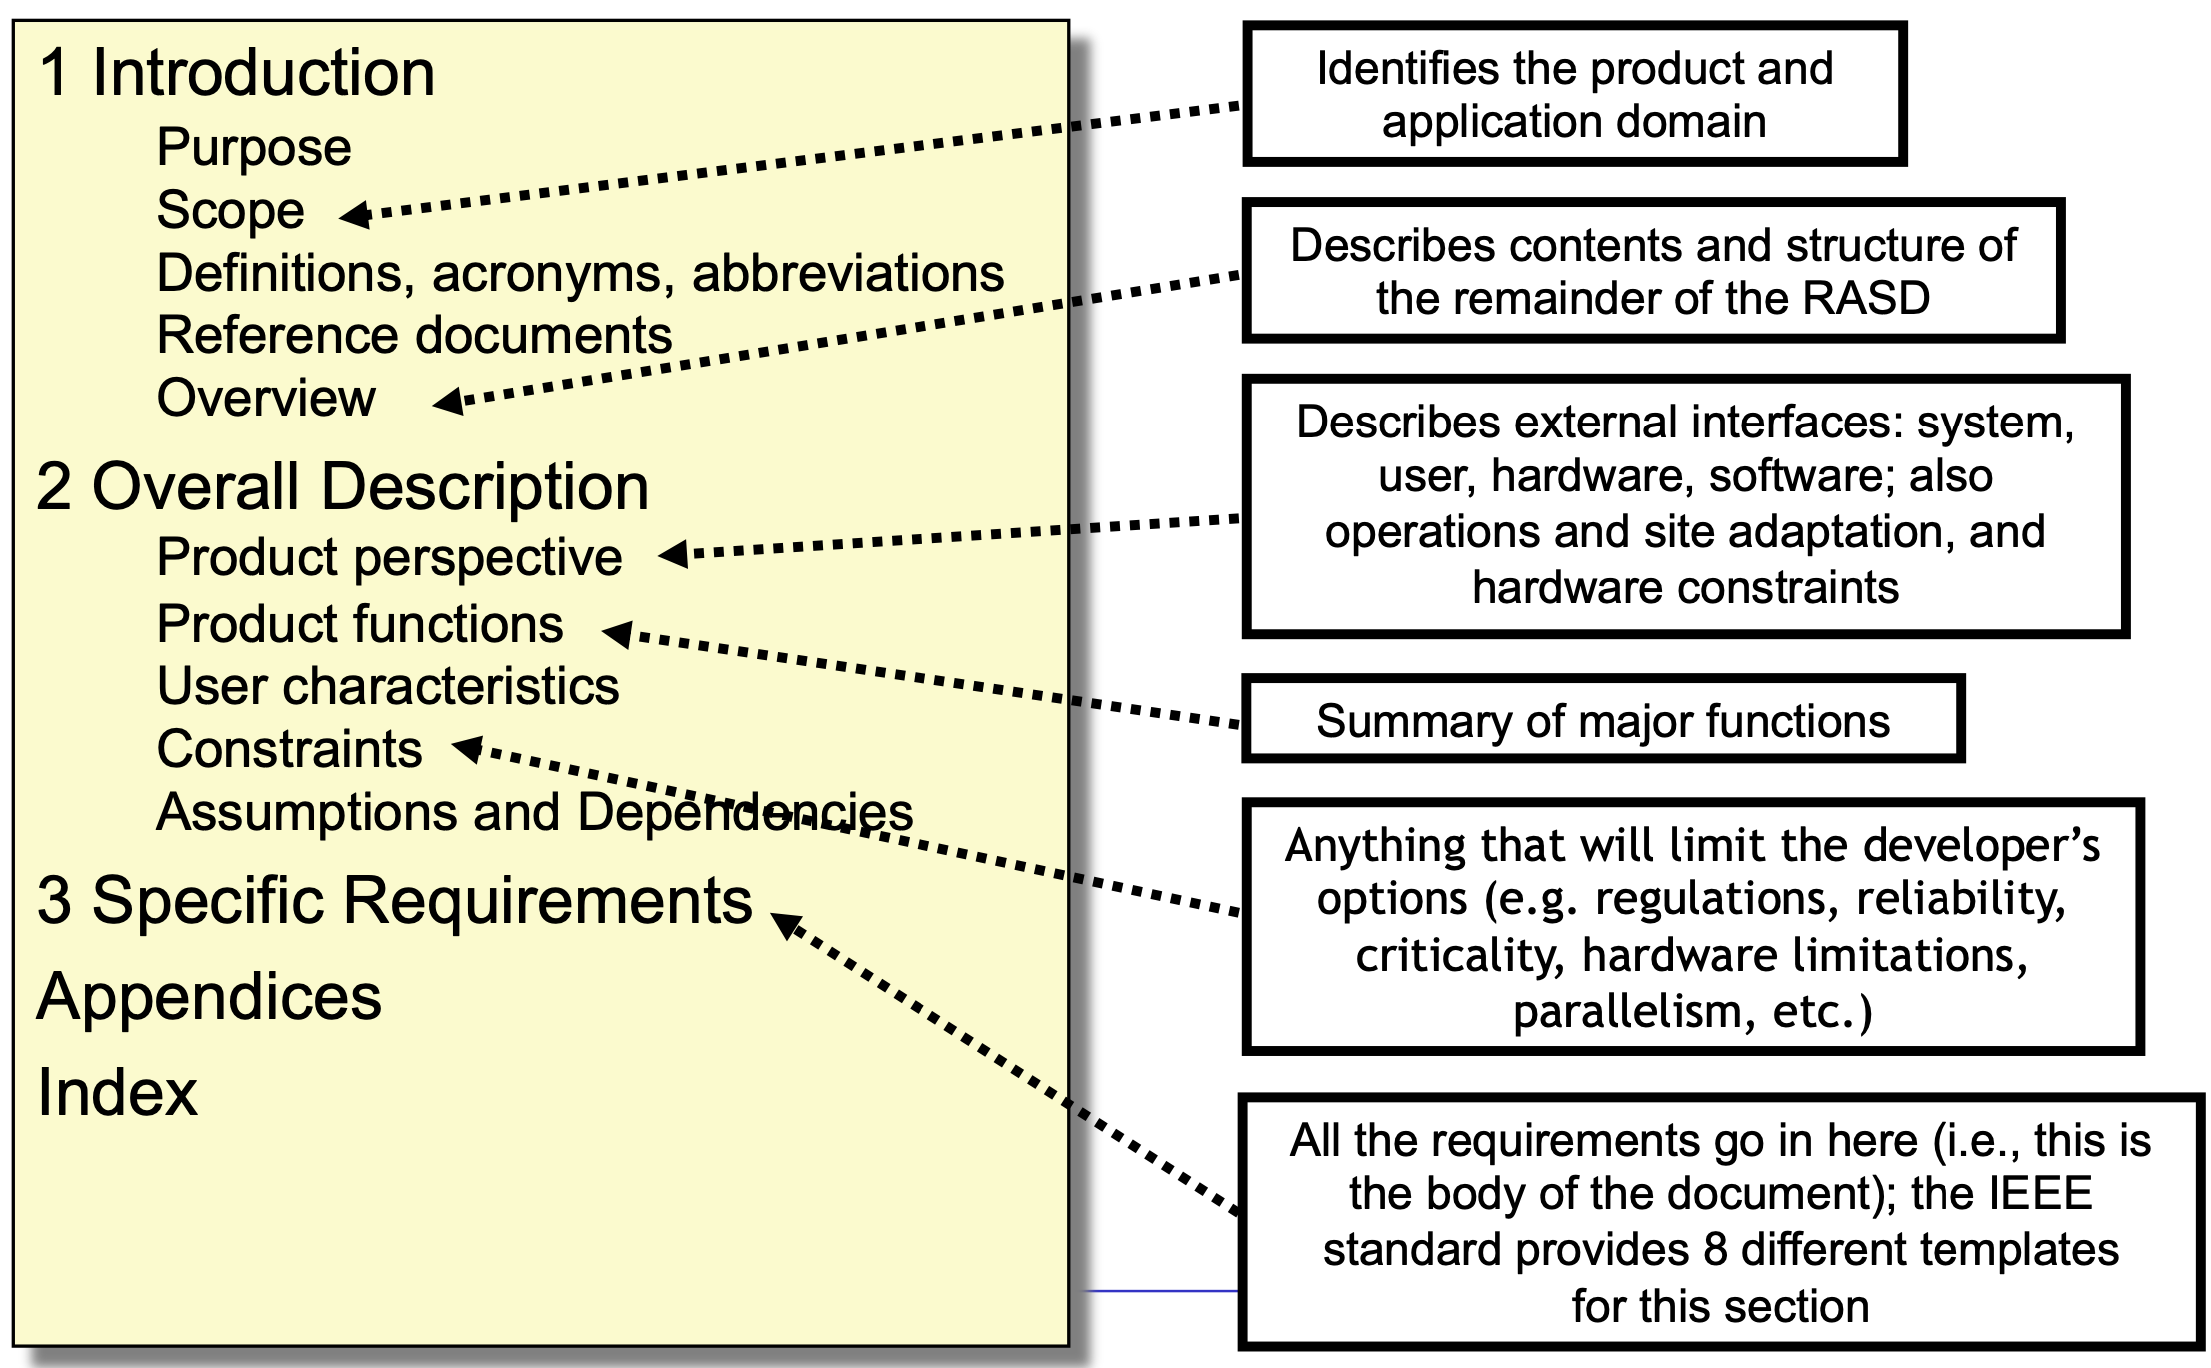
\includegraphics[width=1\linewidth]{images/RASD.png}
        \caption{IEEE standard for RASD}
    \end{figure}
    \par
    The target qualities for a good RASD are: 
    \begin{itemize}
        \item Completeness:
        \begin{itemize}
            \item w.r.t. goals: the requirements are sufficient to satisfy the goals under given domain assumptions: 
            \[Req \land Dom \models Goals\]
            This means that all Goals have been correctly identified, including all relevant quality goals and that the Dom represent valid assumptions; incidental and malicious behaviours have been anticipated. 
            \item w.r.t. inputs: the required software behaviour is specified for all possible inputs
            \item Structural completeness: no TBDs
        \end{itemize}
        \item Pertinence: 
        \begin{itemize}
            \item Each requirement or domain assumption is needed for the satisfaction of some goal. 
            \item Each goal is truly needed by the stakeholders. 
            \item The RASD does not contain items that are unrelated to the definition of requirements.
        \end{itemize}
        \item Consistency: no contradiction in formulation of goals, requirements, and assumptions. 
        \item Unambiguity: 
        \begin{itemize}
            \item Unambiguous vocabulary: every term is defined and used consistently.
            \item Unambiguous assertions: goals, requirements and assumptions must be stated clearly in a way that precludes different interpretations.
            \item Verifiability: a process exists to test satisfaction of each requirement.
            \item Unambiguous responsibilities: the split of responsibilities between the software-to-be and its environment must be clearly indicated. 
        \end{itemize}
        \item Feasibility: the goals and requirements must be realisable within the assigned budget and schedules. 
        \item Comprehensibility: must be comprehensible by all in the target audience.
        \item Good structuring: every item must be defined before it is used.
        \item Modifiability: must be easy to adapt, extend or contract through local modifications and impact of modifying an item should be easy to assess
        \item Traceability: 
        \begin{itemize}
            \item Must indicate sources of goals, requirements and assumptions. 
            \item Must link requirements and assumptions to underlying goals.
            \item Facilitates referencing of requirements in future documentation.
        \end{itemize}
    \end{itemize}

\newpage

\chapter{Software design}
\section{Software architecture}
    \begin{remark}
        The \emph{architecture} of a software system defines that system in terms of computational components ad interactions among those components.
    \end{remark}
    \begin{remark}
        The \emph{software architecture} of a system is the structure of structures of the system, which comprise software elements, the externally visible properties of those elements, and the relationships among them.
    \end{remark}
    In the second definition the most important issues raised are: multiple system structure and externally visible properties of components. This definition does not include: the process, rules and guidelines and architectural styles.
    \par
    Software architecture is really important because: 
    \begin{itemize}
        \item It is the vehicle for stakeholders communication.
        \item it manifests the earliest set of design decisions (constraint on implementation, dictates organizational structure and inhibits or enables quality attributes).
        \item it is a transferable abstraction of a system (product lines share a common architecture, allows for template-based development and basis for training).
    \end{itemize}
\section{Architecture life cycle}
    \begin{figure}
        \centering
        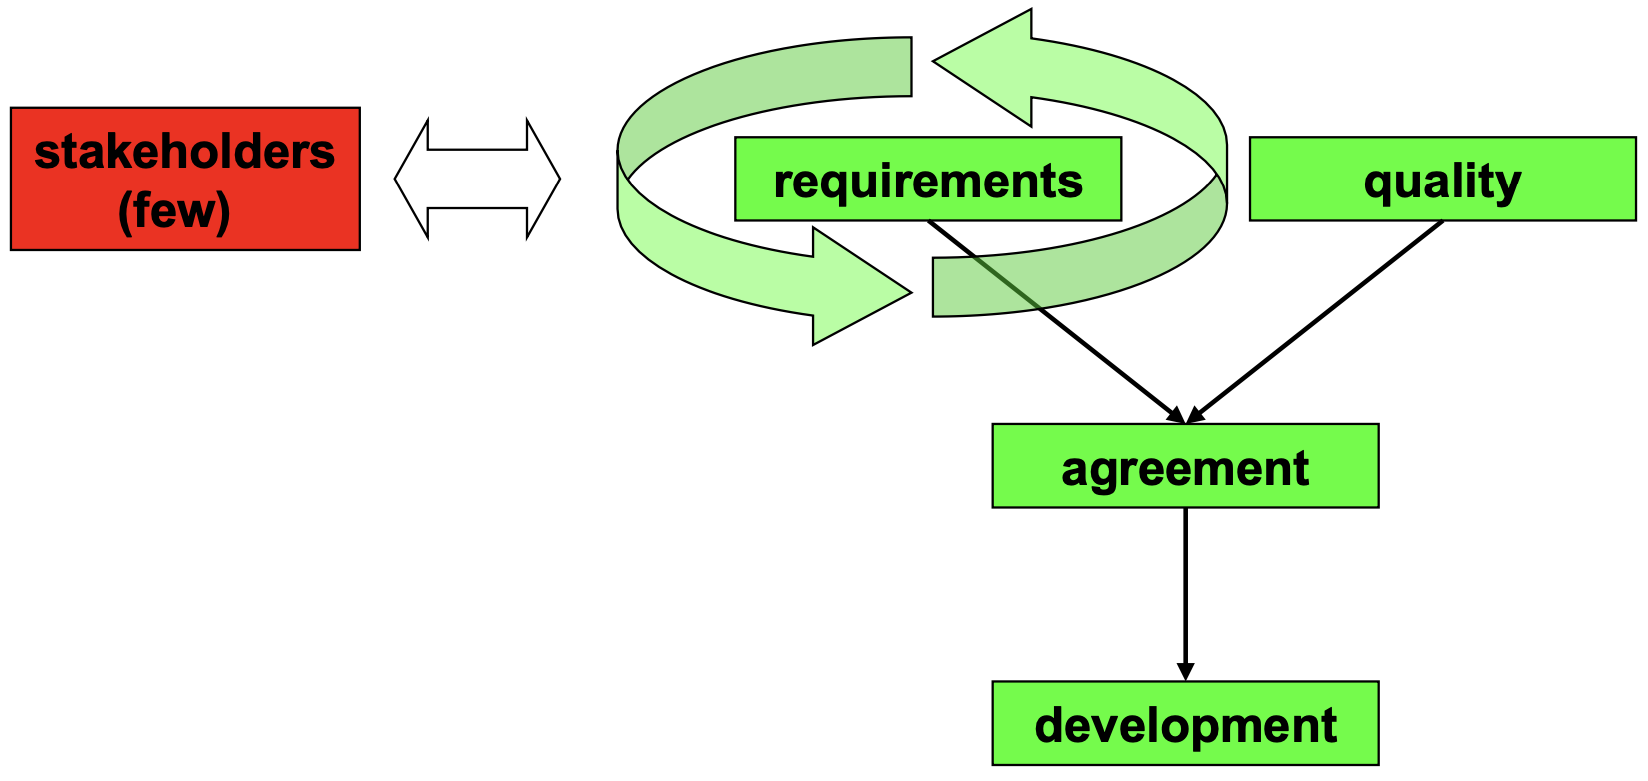
\includegraphics[width=1\linewidth]{images/archlife.png}
        \caption{Pre-architecture life cycle}
    \end{figure}
    The iteration of this life cycle are mainly on functional requirements, only a few stakeholder are involved and no balancing of functional and quality requirements. If we add importance to architecture we have the following characteristics: 
    \begin{itemize}
        \item Iteration on both functional and quality requirements.
        \item Many stakeholder involved.
        \item Balancing of functional and quality requirements.
    \end{itemize}
    \begin{figure}
        \centering
        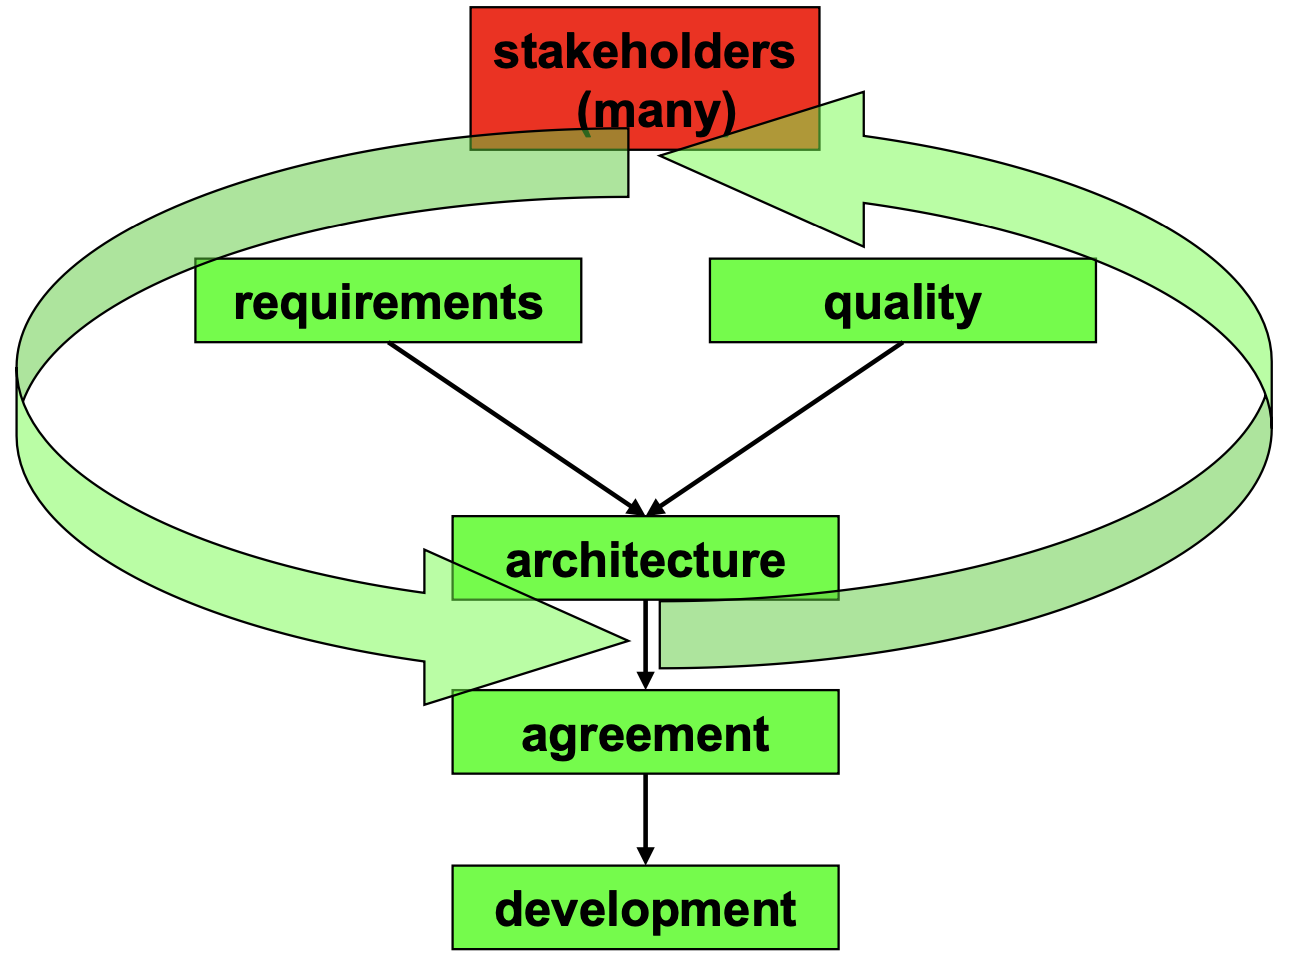
\includegraphics[width=0.5\linewidth]{images/archlife_1.png}
        \caption{Life cycle considering architecture}
    \end{figure}
    In general, a software architecture is intrinsic in the software. 
    \par
    When changes are applied to the code we have an architectural degradation: the changes in the software system are not reflected in the corresponding architectural description. This happens because of: lack of a documented architecture, inadequate processes and supporting tools, developer sloppiness and perception of short deadlines. The degradation can be classified in:
    \begin{itemize}
        \item Drift: the change is not included nor implied by the architecture but it does not necessarily imply its outright violation.
        \item Erosion: the change violates the described architecture.
    \end{itemize}
\section{Software architecture quality and style}
    The notion of quality is central in software architecting: a software architecture is devised to gain insight in the qualities of a system at the earliest possible stage. Some are observable via execution (performance, security, availability, functionality and usability) and some aren't (modifiability, portability, reusability, integrability and testability). 
    \begin{remark}
        An \emph{architectural style} determines the vocabulary of components and connectors that can be used in instances of that style, together with a set of constraints on how they can be combined. These can include topological constraints on architectural descriptions. Other constraints—say, having to do with execution semantics—might also be part of the style definition.
    \end{remark}
    The architectural styles can be: 
    \begin{itemize}
        \item Layered (operative system): the system is organized trough abstraction levels, as a hierarchy of abstract machines. Hierarchy is given by the use relation.
        \item Client-server (distributed applications): they are different processes with well-defined interface (accessible only trough interfaces and they can be defined by a set of hardware/software modules).
        \begin{figure}
            \centering
            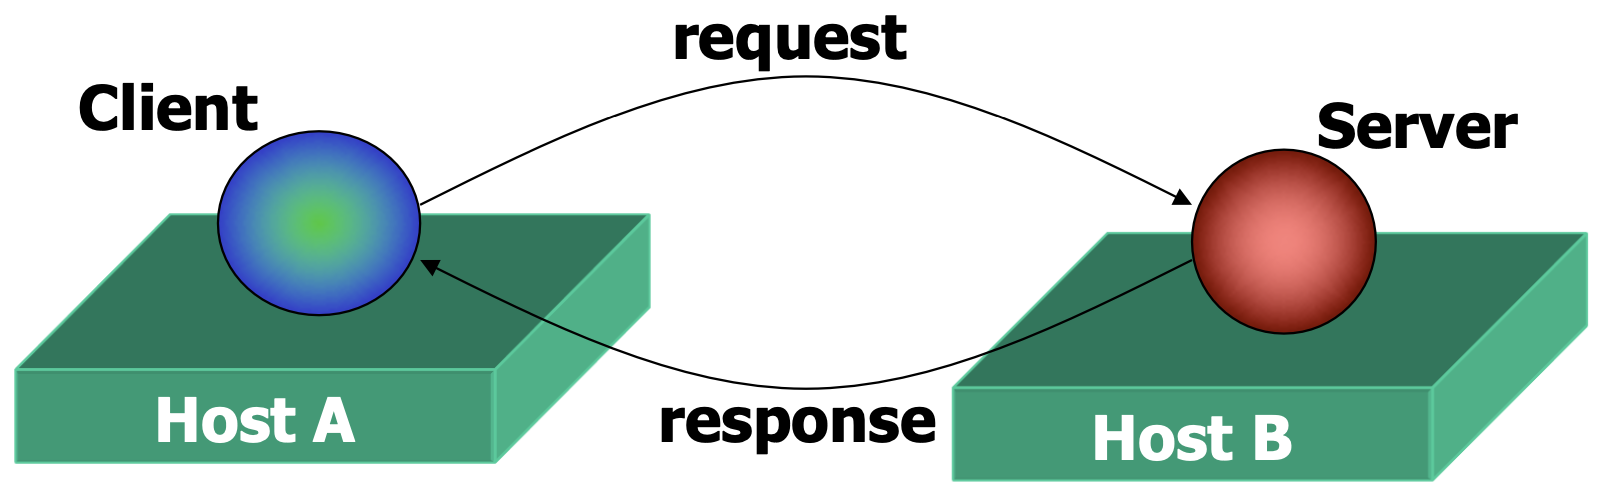
\includegraphics[width=0.5\linewidth]{images/clientserver.png}
            \caption{Client-server architecture general schema}
        \end{figure}
        \item Three-tier architecture: the mid level deals with the application logic. the main advantage is the decoupling of logic and data, logic and presentation.
        \item Event-based systems: the components in this architecture can register to send/receive events that are always broadcasted to all registered components (they don't know who is the sender nor the receiver). Those systems are often called publish-subscribe. This type of architecture allow easy addition/deletion of components and is increasingly used in modern integration strategies. The main problems are about scalability and ordering of events. The main characteristics are: 
        \begin{itemize}
            \item Asynchrony (send and forget).
            \item Reactive (computation driven by receipt of message).
            \item Location/identity abstraction (destination determined by receiver, not sender). 
            \item Loose coupling (senders/receivers added without reconfiguration one-to-many, many-to-one, many-to-many).
        \end{itemize}
        \item Service-oriented architecture (SOA), where the main pros are: 
        \begin{itemize}
            \item Enables reuse of registries and providers across organization boundaries.
            \item Relies on run-time discovery and dynamic binding. 
            \item Service offered through a well-defined Application Programming Interface. 
        \end{itemize}
        But it has also many problems like: dynamic orchestration of discovered services in sot trivial and SOAP protocol is considered too heavy. 
        \begin{figure}
            \centering
            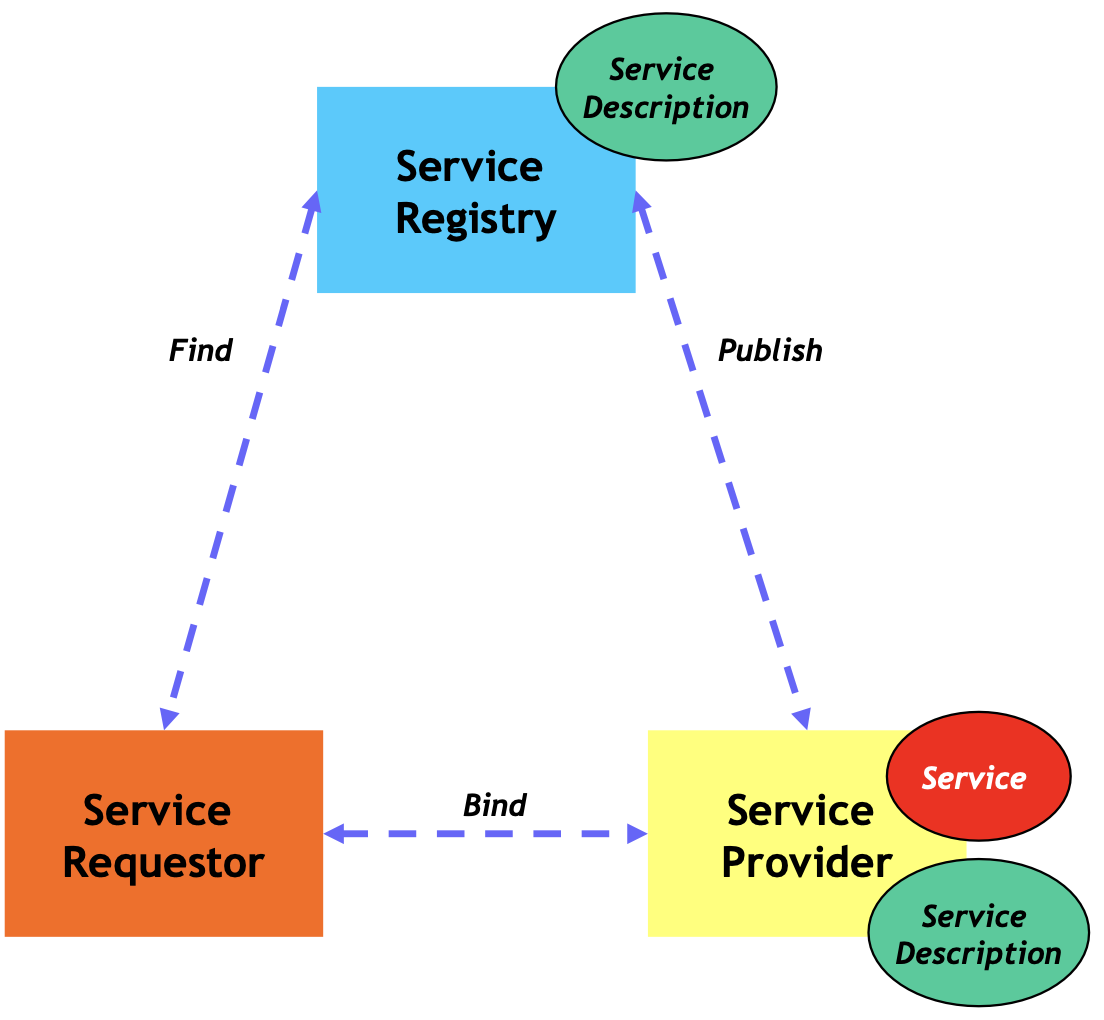
\includegraphics[width=0.5\linewidth]{images/SOA.png}
            \caption{Service-oriented architecture schema}
        \end{figure}
        \item Micro-service architecture: monolithic systems are decomposed into small specialized services and deal with a single bounded context in the target domain. The micro-service architectural style is an approach to developing a single application as a suite of small services, each running in its own process and communicating with lightweight mechanisms, often an HTTP resource API. This type of architecture solves the following problem with the monolithic systems: issues with frequent deployment, overloaded containers, obstacle to scaling development, may lead to availability issues and requires long-term commitment to a technology stack. With this architecture it's possible to use different technology for each part of the complete system. This architecture is resilient because every module (that can use different technology and developing teams) is detached partially from the others and also highly scalable. The main problems of this method are that we deal with distributed systems and that the decomposition of monolithic systems are complex and needs collaboration.
    \end{itemize}
\section{Software design description and principles}  
    The IEEE defines two standards for the architectural model: 
    \begin{itemize}
        \item IEEE Standard for Information Technology — Systems Design — Software Design Descriptions.
        \item IEEE Standard for Systems and software engineering — Architecture description (manner in which architectural descriptions of systems are organized and expressed).
    \end{itemize}
    According to IEEE standards a SDD needs to have: 
    \begin{itemize}
        \item Identification of the SDD (date, authors, organization,$\dots$).
        \item Description of design stakeholders.
        \item Description of design concerns.
        \item Selected design viewpoints.
        \item Design views.
        \item Design overlays.
        \item Design rationale.
    \end{itemize}
    The eleven design principles are: 
    \begin{enumerate}
        \item Divide and conquer: simplify the problems with smaller ones.
        \item Keep the level of abstraction as high as possible: ensure that your designs allow you to hide or defer consideration of details, thus reducing complexity.
        \item Increase cohesion where possible.
        \item Reduce coupling where possible.
        \item Design for reusability: design the various aspects of your system so that they can be used again in other contexts.
        \item Reuse existing designs and code: design with reuse is complementary to design for reusability.
        \item Design for flexibility: actively anticipate changes that a design may have to undergo in the future, and prepare for them. 
        \item Anticipate obsolescence: plan for changes in the technology or environment so the software will continue to run or can be easily changed. 
        \item Design for portability: have the software run on as many platforms as possible. 
        \item Design for testability: take steps to make testing easier.
        \item Design defensively: be careful when you trust how others will try to use a component you are designing.
    \end{enumerate}
\section{The design process}
    \begin{remark}
        Defining the software architecture or design is a problem-solving process whose objective is to find and describe a way to implement the system functional requirements while respecting the constraints imposed by the quality, platform and process requirements (including the budget) and while adhering to general principles of good quality.
    \end{remark}
    The possible approaches are: 
    \begin{itemize}
        \item Top-down: first design design the very high level structure of the system, then gradually work down to detailed decisions about low-level constructs and finally arrive at detailed decisions such as the format of particular data items and the individual algorithms that will be used.
        \item Bottom-up: make decisions about reusable low-level utilities then decide how these will be put together to create high-level constructs.
        \item Mixed approach: create the structure with top-down and define reusable components with bottom-up methods.
    \end{itemize}
    The designer is faced with a series of designed issues and needs to select the best option for every problem that encounters. The space of the possible designs that could be achieved by choosing different sets of alternatives is often called the design space. 
    










    

    
\end{document}